\documentclass[10pt,a4paper]{article}
\usepackage[margin=1.4cm]{geometry}
% common.tex - shared preamble for all ELL7282 A2 documents
\usepackage[T1]{fontenc}
\usepackage{lmodern}
\usepackage{amsmath,amssymb}
\usepackage{booktabs,longtable,tabularx,array,multirow}
\usepackage[table]{xcolor}
\usepackage{bytefield}
\usepackage{tikz}
\usetikzlibrary{arrows.meta,positioning,fit,calc,shapes.geometric}
\usepackage{pdflscape}
\usepackage{enumitem}
\usepackage{caption}
\usepackage[hidelinks]{hyperref}
\setlist{nosep,leftmargin=1.4em}
\setlength{\parskip}{3pt}
\setlength{\parindent}{0pt}

\newcommand{\project}{WM-8 five-stage pipelined washing-machine microcontroller}
\newcommand{\course}{ELL7282/ELL782 Introduction to Computer Architecture -- Assignment 2}
\newcommand{\pass}{\textcolor{green!45!black}{\textbf{PASS}}}
\newcommand{\fail}{\textcolor{red!75!black}{\textbf{FAIL}}}
% invalid (V=0) pipeline entry: grey with an empty-set marker
\newcommand{\bub}[1]{\textcolor{black!45}{$\varnothing$\,\texttt{#1}}}
\newcommand{\sig}[1]{\texttt{#1}}
\newcommand{\hex}[1]{\texttt{0x#1}}

% cycle-trace table (used by generated/trace*.tex)
\newenvironment{tracetab}{%
  \scriptsize\setlength{\tabcolsep}{2.5pt}\renewcommand{\arraystretch}{1.15}%
  \begin{longtable}{r p{3.0cm} p{3.0cm} p{3.0cm} p{3.0cm} p{3.0cm} c c c c p{4.6cm}}
  \toprule
  Cyc & IF (fetch PC) & ID (IF/ID) & EX (ID/EX) & MEM (EX/MEM) & WB (MEM/WB) &
  Stall & Flush & Fwd A & Fwd B & Architectural writes (commit at end of cycle)\\
  \midrule\endhead
  \bottomrule\endfoot}{%
  \end{longtable}}

% validation table (used by generated/val_g*.tex)
\newenvironment{valtab}{%
  \footnotesize\renewcommand{\arraystretch}{1.2}%
  \begin{longtable}{|p{0.6cm}|p{3.7cm}|p{4.2cm}|p{5.6cm}|p{1.0cm}|}
  \hline
  \rowcolor{black!8}\textbf{ID} & \textbf{Initial inputs / state, stimulus} & \textbf{Expected result} &
  \textbf{Observed result} & \textbf{P/F}\\ \hline\endhead}{%
  \end{longtable}}

% program listing (used by generated/listing_*.tex)
\newenvironment{listtab}{%
  \footnotesize\setlength{\tabcolsep}{4pt}\renewcommand{\arraystretch}{1.05}%
  \begin{longtable}{l l c l l p{6.2cm}}
  \toprule
  Addr & Hex & Fmt & Label & Assembly & Comment\\
  \midrule\endhead
  \bottomrule\endfoot}{%
  \end{longtable}}

\tikzset{
  blk/.style={draw,thick,fill=blue!6,rounded corners=2pt,align=center,font=\scriptsize,minimum height=7mm,inner sep=2pt},
  mem/.style={draw,thick,fill=orange!12,align=center,font=\scriptsize,minimum height=9mm,inner sep=2pt},
  preg/.style={draw,thick,fill=black!12,minimum width=4mm,minimum height=52mm,align=center,font=\tiny},
  sigl/.style={-{Stealth[length=2mm]},thick},
  fwdl/.style={-{Stealth[length=2mm]},thick,red!70!black},
  ctl/.style={-{Stealth[length=2mm]},thick,dashed,blue!60!black},
  lab/.style={font=\tiny,inner sep=1pt}
}
\begin{document}
\begin{center}
{\Large\textbf{Architecture of the WM-8 Pipelined Microcontroller}}\\[1pt]
\course
\end{center}
\vspace{-2mm}
\section*{1. Block diagram}
\begin{center}\resizebox{\textwidth}{!}{%
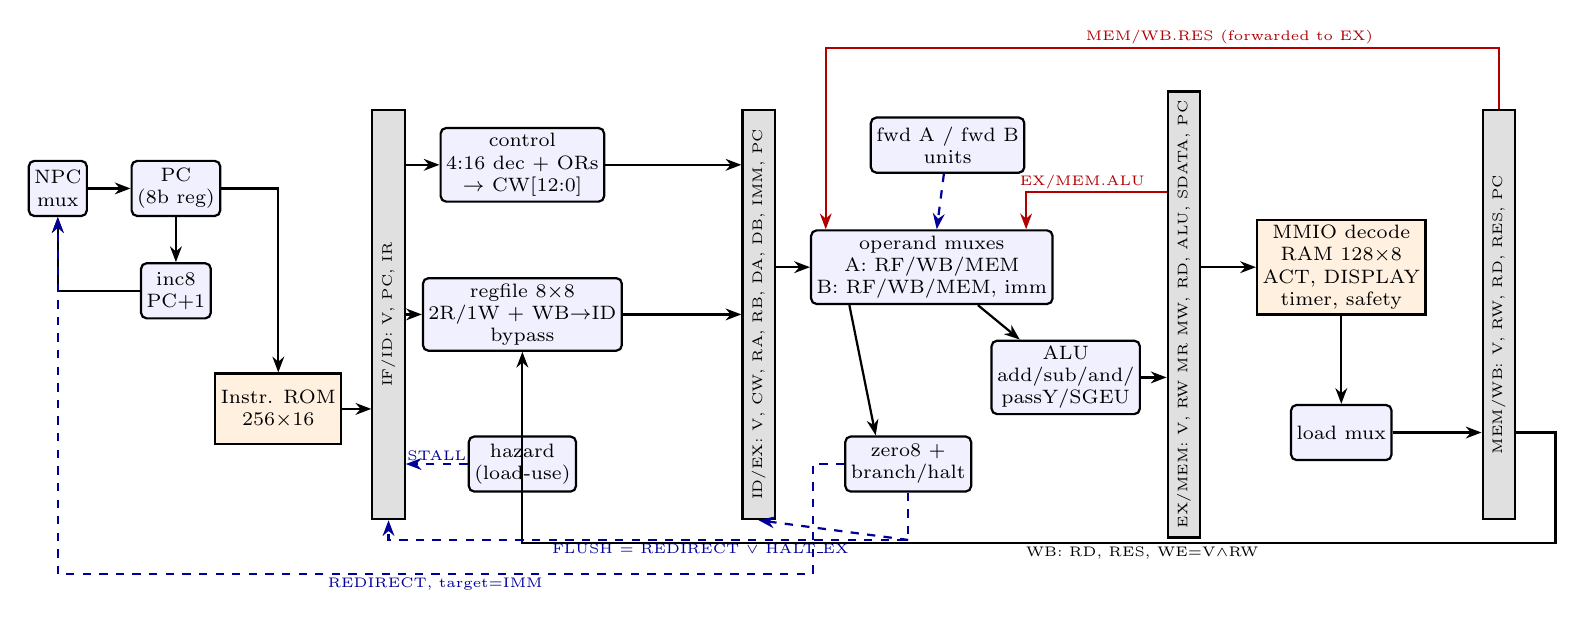
\begin{tikzpicture}[x=1cm,y=1cm]
% pipeline registers
\node[preg] (r1) at (3.3,0) {\rotatebox{90}{IF/ID: V, PC, IR}};
\node[preg] (r2) at (8.0,0) {\rotatebox{90}{ID/EX: V, CW, RA, RB, DA, DB, IMM, PC}};
\node[preg] (r3) at (13.4,0) {\rotatebox{90}{EX/MEM: V, RW MR MW, RD, ALU, SDATA, PC}};
\node[preg] (r4) at (17.4,0) {\rotatebox{90}{MEM/WB: V, RW, RD, RES, PC}};
% IF
\node[blk] (pc) at (0.6,1.6) {PC\\(8b reg)};
\node[blk] (inc) at (0.6,0.3) {inc8\\PC+1};
\node[blk] (npc) at (-0.9,1.6) {NPC\\mux};
\node[mem] (rom) at (1.9,-1.2) {Instr. ROM\\256$\times$16};
% ID
\node[blk] (ctl) at (5.0,1.9) {control\\4:16 dec + ORs\\$\rightarrow$ CW[12:0]};
\node[blk] (rf) at (5.0,0.0) {regfile 8$\times$8\\2R/1W + WB$\rightarrow$ID\\bypass};
\node[blk] (hz) at (5.0,-1.9) {hazard\\(load-use)};
% EX
\node[blk] (fw) at (10.4,2.15) {fwd A / fwd B\\units};
\node[blk] (mx) at (10.2,0.6) {operand muxes\\A: RF/WB/MEM\\B: RF/WB/MEM, imm};
\node[blk] (alu) at (11.9,-0.8) {ALU\\add/sub/and/\\passY/SGEU};
\node[blk] (br) at (9.9,-1.9) {zero8 +\\branch/halt};
% MEM
\node[mem] (io) at (15.4,0.6) {MMIO decode\\RAM 128$\times$8\\ACT, DISPLAY\\timer, safety};
\node[blk] (lm) at (15.4,-1.5) {load mux};
% arrows
\draw[sigl] (npc) -- (pc);
\draw[sigl] (pc) -- (inc);
\draw[sigl] (inc.west) -| (npc.south);
\draw[sigl] (pc.east) -| (rom.north);
\draw[sigl] (rom.east) -- (r1.west|-rom.east);
\draw[sigl] (r1.east|-ctl) -- (ctl);
\draw[sigl] (r1.east|-rf) -- (rf);
\draw[sigl] (ctl) -- (r2.west|-ctl);
\draw[sigl] (rf) -- (r2.west|-rf);
\draw[sigl] (r2.east|-mx) -- (mx);
\draw[sigl] (mx) -- (alu);
\draw[sigl] ($(mx.south west)+(0.5,0)$) -- ($(br.north west)+(0.4,0)$);
\draw[sigl] (alu) -- (r3.west|-alu);
\draw[sigl] (r3.east|-io) -- (io);
\draw[sigl] (io) -- (lm);
\draw[sigl] (lm) -- (r4.west|-lm);
\draw[sigl] (r4.east|-0,-1.5) -- ++(0.5,0) -- ++(0,-1.4) -| node[lab,pos=0.2,below]{WB: RD, RES, WE=V$\wedge$RW} (rf.south);
% forwarding
\draw[fwdl] (r3.west|-0,1.55) -| node[lab,above,pos=0.3]{EX/MEM.ALU} ($(mx.north east)+(-0.35,0)$);
\draw[fwdl] (r4.north) |- node[lab,above,pos=0.7]{MEM/WB.RES (forwarded to EX)} ($(mx.north west)+(0.2,2.3)$) -- ($(mx.north west)+(0.2,0)$);
% control
\draw[ctl] (br.west) -- ++(-0.4,0) |- node[lab,pos=0.75,below]{REDIRECT, target=IMM} (-0.9,-3.3) -- (npc.south);
\draw[ctl] (hz.west) -- node[lab,above]{STALL} (r1.east|-hz);
\draw[ctl] (br.south) -- ++(0,-0.6) -| node[lab,pos=0.2,below]{FLUSH = REDIRECT $\vee$ HALT\_EX} (r1.south);
\draw[ctl] (fw) -- (mx);
\draw[ctl] ($(br.south)+(0,-0.6)$ -| r2.south) -- (r2.south);
\end{tikzpicture}}
\end{center}
\vspace{-2mm}
{\footnotesize Grey bars: pipeline registers (built from Logisim Registers, one per field, all clocked by the single global
clock, asynchronous \texttt{CLR}=\texttt{RESET}). Red: forwarding paths into EX. Dashed: hazard and control-transfer
signals. Every multiplexer, decoder, comparator, adder, incrementer and the ALU is a gate-level sub-circuit
(\texttt{mux2\_8}, \texttt{mux4\_8}, \texttt{mux8\_8}, \texttt{dec3to8}, \texttt{dec4to16}, \texttt{eq3}, \texttt{eq8}, \texttt{zero8},
\texttt{fa1}/\texttt{add8}, \texttt{ha1}/\texttt{inc8}, \texttt{and8en}, \texttt{alu8}). The Plexers and Arithmetic libraries are not
even loaded in the \texttt{.circ}.}

\section*{2. Pipeline registers and control word}
\begin{center}
\scriptsize\renewcommand{\arraystretch}{1.12}
\begin{tabular}{|l|p{11.6cm}|r|}
\hline\rowcolor{black!8}
\textbf{Register} & \textbf{Fields (Logisim register label: width)} & \textbf{bits}\\ \hline
PC & \texttt{PC}:8 (enable \texttt{PC\_EN}) & 8\\ \hline
IF/ID & \texttt{IFID.V}:1, \texttt{IFID.PC}:8, \texttt{IFID.IR}:16 (common enable \texttt{IFID\_EN}) & 25\\ \hline
ID/EX & \texttt{IDEX.V}:1, \texttt{IDEX.CW}:13, \texttt{IDEX.RA}:3 (=destination), \texttt{IDEX.RB}:3, \texttt{IDEX.DA}:8, \texttt{IDEX.DB}:8,
  \texttt{IDEX.IMM}:8, \texttt{IDEX.PC}:8 & 52\\ \hline
EX/MEM & \texttt{EXMEM.V}:1, \texttt{EXMEM.CTRL}:3 (\texttt{RW,MR,MW}), \texttt{EXMEM.RD}:3, \texttt{EXMEM.ALU}:8 (result or address),
  \texttt{EXMEM.SDATA}:8 (forwarded store data), \texttt{EXMEM.PC}:8 & 31\\ \hline
MEM/WB & \texttt{MEMWB.V}:1, \texttt{MEMWB.RW}:1, \texttt{MEMWB.RD}:3, \texttt{MEMWB.RES}:8 (ALU or load data), \texttt{MEMWB.PC}:8 & 21\\ \hline
other & \texttt{HALTED}:1; regfile \texttt{R0}--\texttt{R7}:8 each; MMIO \texttt{ACT}:8, \texttt{DISPLAY}:8; timer \texttt{COUNT}, \texttt{LIMIT}:8,
  \texttt{EN}, \texttt{MATCH}:1; safety \texttt{TRIP}, \texttt{START\_PREV}:1 & \\ \hline
\end{tabular}
\end{center}
The \texttt{PC} fields are carried only for observation (pipeline monitor and traces). \texttt{CW} bits:
\texttt{RW}(0) register write, \texttt{MR}(1) load, \texttt{MW}(2) store, \texttt{UA}(3)/\texttt{UB}(4) instruction reads
\texttt{ra}/\texttt{rb}, \texttt{YI}(5) ALU-Y=imm, \texttt{AOP}(7:6) result select, \texttt{SB}(8) subtract, \texttt{BZ}(9),
\texttt{BNZ}(10), \texttt{JP}(11), \texttt{HT}(12). The full per-opcode table is in \texttt{isa.pdf}.

\section*{3. Stage operation}
\textbf{IF}: \texttt{I\_ADDR}=\texttt{PC}; the ROM word is latched into IF/ID. \texttt{NPC} = \texttt{REDIRECT} ?
\texttt{IDEX.IMM} : \texttt{PC}+1. \textbf{ID}: \texttt{IR} is split into \texttt{OP}, \texttt{RA}=\texttt{IR[11:9]},
\texttt{RB}=\texttt{IR[8:6]}, \texttt{IMM}=\texttt{IR[7:0]}. The control decoder, both register reads and the hazard check
run in parallel. The register file writes on the clock edge, and a WB$\rightarrow$ID bypass
(\texttt{WE}$\wedge$\texttt{WA}=\texttt{RA} ? \texttt{WD} : \texttt{R[RA]}, likewise for \texttt{RB}) makes a write-back
visible to an ID read in the same cycle. \textbf{EX}: operands are forwarded, \texttt{Y} = \texttt{YI} ? \texttt{IMM} :
\texttt{opB}, the ALU computes, and branch, jump and \texttt{HALT} are resolved. \texttt{LD}/\texttt{ST} pass \texttt{opB}
through the ALU as the address, and \texttt{opA} becomes the store data. \textbf{MEM}: one-cycle access to the
memory-mapped bus, and \texttt{RES} = \texttt{MR} ? \texttt{D\_RDATA} : \texttt{ALU}. \textbf{WB}: \texttt{R[RD]}
$\leftarrow$ \texttt{RES} when \texttt{MEMWB.V}$\wedge$\texttt{MEMWB.RW}.

\section*{4. Forwarding, stall and flush logic (all signals are gate level)}
\begin{center}\footnotesize\setlength{\tabcolsep}{3pt}
\begin{tabular}{r l}
\texttt{USE\_A} &= \texttt{IDEX.V} $\wedge$ \texttt{UA}, \quad \texttt{USE\_B} = \texttt{IDEX.V} $\wedge$ \texttt{UB} \hfill (only real sources are forwarded)\\
\texttt{EXM\_A} &= \texttt{USE\_A} $\wedge$ \texttt{EXMEM.V} $\wedge$ \texttt{EXMEM.RW} $\wedge$ (\texttt{EXMEM.RD} = \texttt{IDEX.RA})\\
\texttt{F\_EXMEM\_A} &= \texttt{EXM\_A} $\wedge$ $\lnot$\texttt{EXMEM.MR} \hfill (a load in EX/MEM is never forwarded)\\
\texttt{F\_MEMWB\_A} &= \texttt{USE\_A} $\wedge$ \texttt{MEMWB.V} $\wedge$ \texttt{MEMWB.RW} $\wedge$ (\texttt{MEMWB.RD} = \texttt{IDEX.RA}) $\wedge$ $\lnot$\texttt{EXM\_A} \hfill (youngest writer wins)\\
\texttt{opA} &= \texttt{F\_EXMEM\_A} ? \texttt{EXMEM.ALU} : (\texttt{F\_MEMWB\_A} ? \texttt{MEMWB.RES} : \texttt{IDEX.DA}) \hfill (same for B with \texttt{RB})\\[3pt]
\texttt{STALL\_RAW} &= \texttt{IFID.V} $\wedge$ \texttt{IDEX.V} $\wedge$ \texttt{IDEX.MR} $\wedge$
   [(\texttt{UA}$\wedge$\texttt{RA}=\texttt{IDEX.RA}) $\vee$ (\texttt{UB}$\wedge$\texttt{RB}=\texttt{IDEX.RA})]\\
\texttt{REDIRECT} &= \texttt{IDEX.V} $\wedge$ [\texttt{JP} $\vee$ (\texttt{BZ}$\wedge$\texttt{opA}=0) $\vee$ (\texttt{BNZ}$\wedge$\texttt{opA}$\neq$0)],
  \quad \texttt{HALT\_EX} = \texttt{IDEX.V} $\wedge$ \texttt{HT}\\
\texttt{FLUSH} &= \texttt{REDIRECT} $\vee$ \texttt{HALT\_EX}, \quad \texttt{STALL} = \texttt{STALL\_RAW} $\wedge$ $\lnot$\texttt{FLUSH} (flush has priority)\\
\texttt{PC\_EN} &= \texttt{REDIRECT} $\vee$ $\lnot$(\texttt{STALL\_RAW} $\vee$ \texttt{HALT\_EX} $\vee$ \texttt{HALTED})\\
\texttt{IFID\_EN} &= $\lnot$\texttt{STALL\_RAW} $\vee$ \texttt{FLUSH}, \quad \texttt{IFID.V}$\leftarrow$ $\lnot$(\texttt{FLUSH} $\vee$ \texttt{HALTED})\\
\texttt{IDEX.V} &$\leftarrow$ \texttt{IFID.V} $\wedge$ $\lnot$\texttt{STALL\_RAW} $\wedge$ $\lnot$\texttt{FLUSH};\quad
  \texttt{EXMEM.V}$\leftarrow$\texttt{IDEX.V};\quad \texttt{MEMWB.V}$\leftarrow$\texttt{EXMEM.V}\\
\end{tabular}
\end{center}
Load-use: \texttt{PC} and IF/ID hold for one cycle, and ID/EX receives a bubble (\texttt{V}=0) while EX/MEM and MEM/WB advance. The
consumer then takes the load value from MEM/WB, so it waits exactly one cycle. Distance-2 consumers are forwarded
from MEM/WB, and distance-3 consumers read through the WB$\rightarrow$ID bypass. A taken branch or jump costs two cycles: the
wrong-path entries in IF/ID and ID/EX are invalidated at the edge that loads the target. A load-use stall needs a load in
EX and a redirect needs a branch in EX, so they cannot come from the same instruction. The \texttt{FLUSH} term still
gives the redirect explicit priority. Architectural writes are gated by \texttt{V}: register file
\texttt{WB\_WE}=\texttt{MEMWB.V}$\wedge$\texttt{RW}, data bus \texttt{D\_WE}=\texttt{EXMEM.V}$\wedge$\texttt{MW}. MEM never
stalls, so each store is presented to the bus for exactly one edge.

\section*{5. Reset and HALT}
The single \texttt{RESET} input drives the asynchronous \texttt{CLR} of every pipeline, control, I/O, timer and safety register.
This gives \texttt{PC}=0, all \texttt{V}=0, \texttt{HALTED}=0, \texttt{ACT} and \texttt{DISPLAY} = 0 (all actuator requests off), a cleared
and disabled timer (\texttt{COUNT}, \texttt{LIMIT}, \texttt{EN} and \texttt{MATCH} all 0) and \texttt{TRIP}=0. The register file and RAM are
deliberately \emph{not} cleared. When a valid \texttt{HALT} is in EX, \texttt{HALT\_EX} freezes the PC, invalidates IF/ID and
ID/EX, and sets the \texttt{HALTED} flip-flop (D=1, EN=\texttt{HALT\_EX}). After that, IF/ID receives \texttt{V}=0 every cycle and
the PC stays frozen. Older instructions in EX/MEM and MEM/WB complete, and the \texttt{HALT} itself drains with no write.
Only \texttt{RESET} clears \texttt{HALTED}. A \texttt{HALT} on a squashed path is invalid before it reaches EX and is ignored.
The timer and the safety logic keep running while the CPU is stalled or halted.

\section*{6. Safety interlock (sub-circuit \texttt{safety})}
\begin{center}\small
\texttt{ActualMotorEnable} = \texttt{REQ} $\wedge$ \texttt{DOOR\_CLOSED} $\wedge$ $\lnot$\texttt{TRIP}\qquad
(\texttt{REQ} = \texttt{ACT[2]}, i.e.\ the CPU \texttt{MOTOR\_EN} request)\\
\texttt{TRIP}$^+$ = (\texttt{REQ} $\wedge$ $\lnot$\texttt{DOOR\_CLOSED}) $\vee$ (\texttt{TRIP} $\wedge$ $\lnot$\texttt{REARM}),\quad
\texttt{REARM} = $\lnot$\texttt{REQ} $\wedge$ \texttt{DOOR\_CLOSED} $\wedge$ \texttt{START} $\wedge$ $\lnot$\texttt{START\_PREV}
\end{center}
\texttt{TRIP} and \texttt{START\_PREV} (which samples \texttt{START} every cycle) are 1-bit Logisim Registers on the global
rising edge. Their clear input is \texttt{RESET} and they have no enable, so they sample every cycle independently of the CPU.
\texttt{TRIP} is set at the first edge at which the door is sampled open while the motor request is 1. The output AND gate is
combinational, so opening the door drops \texttt{ActualMotorEnable} immediately, without waiting for that edge or for software. Once
set, \texttt{TRIP} holds even after the door recloses, so a cleared door sensor alone can never restart the motor. It clears
only at an edge where software has removed the request (\texttt{REQ}=0), the door is closed, and a new
\texttt{START} 0$\rightarrow$1 transition is detected (\texttt{START\_PREV}=0, \texttt{START}=1). Set and re-arm need opposite
values of \texttt{REQ}, so they can never conflict. The path from \texttt{ACT[2]} to the output is a latch written only by
valid MEM-stage stores, so flushed instructions cannot affect it. A faulty program can still request the motor, but can never
assert it while the door is open or \texttt{TRIP}=1. The software reads \texttt{TRIP} and the gated output in
\texttt{IN\_STATUS[5:4]}.

\section*{7. Clocking and Logisim implementation notes}
There is one global rising-edge clock. No clock is gated: all conditional updates use the Register \texttt{EN} input, and the RAM
uses its \texttt{WE} input. Clock skew between hierarchy levels in Logisim (at most 2 sub-circuit boundaries, each a 1-unit pin delay) is
far smaller than the register clock-to-output delay, so every state element samples pre-edge values. The sub-circuit hierarchy
is: \texttt{main} $\rightarrow$ \texttt{cpu} (\texttt{control}, \texttt{regfile}, \texttt{hazard}, 2$\times$\texttt{fwd},
\texttt{alu8}, muxes) and \texttt{mmio} (\texttt{timer8}, \texttt{safety}, decoders, \texttt{and8en} read multiplexer), with ROM
and RAM at the top level so that images are easy to load and inspect. Inside the sub-circuits, every port goes through a short wire
stub to a labelled tunnel, so each net name in this document appears as a tunnel label in the schematic.
\end{document}
